\subsection{\label{sec:fiducial}Fiducial Region Selection}

We derived \emph{Geometric fiducial cuts} for the g12 data, which are cuts based on the exclusion of events laying outside regions where acceptance is well behaved and reliably reproduced in simulation. Such regions for all g12 data are expressed as an upper and lower limit of the difference in azimuthal angle between the center of a given sector, and a particle track.  Because of the hyperbolic geometry of CLAS and the presence of the toroidal magnetic field, the fiducial boundaries on the angle $\phi$ are functions of momentum ($p$), charge, and polar angle ($\theta$) of each track. The boundaries were evaluated separately in each sector, nominally defined as the $\phi$ values in which occupancy drops below 50\% of that in the respective sector's flat region. The flat regions were defined as $-10^{\circ} < \phi < 10^{\circ}$. The nominal upper and lower $\phi$ limits depend strongly on particle charge, $p$ and $\theta$, hence the need for functional characterization and extrapolation.

In order to determine the fiducial limits for charged hadrons, a sample of exclusive \mbox{γ p$\to$p \π[+] \π[-]} events were sliced into $5\times15\times6$ bins in $p$, $\theta$, and sector respectively. The $\phi$ distributions for \π[+] and \π[-] were plotted separately in each bin. The upper and lower $\phi$ limits of these \emph{first-generation} plots were found according to the nominal fiducial definition of 50\% occupancy as illustrated in Fig.~\ref{gen12}. The results from the first-generation fits were represented in \emph{second-generation} plots of $\phi_{min}$ and $\phi_{max}$ vs $\theta$ as also shown in Fig.~\ref{gen12}.  The data in the second-generation plots were fit with hyperbolas, chosen since they replicate the projection of the detector.  Second-generation fitting parameters were then plotted vs $p$ in \emph{third-generation} plots. These third generation plots were fit to power functions as shown in Fig.~\ref{gen3}. Results of the third-generation fits define the sought after functional form $\phi_{min}(\theta,p)$ and $\phi_{max}(\theta,p)$ for each sector. The sector integrated results for positive and negative hadron tracks compose the nominal fiducial region. \emph{Tight cuts} and \emph{loose cuts} were defined as a contraction and expansion respectively, by $4^\circ$ from the nominal fiducial cuts. Figs.~\ref{figures/fiducial/fid2}-\ref{figures/fiducial/fid5} show the effects of the cuts.

\begin{figure}
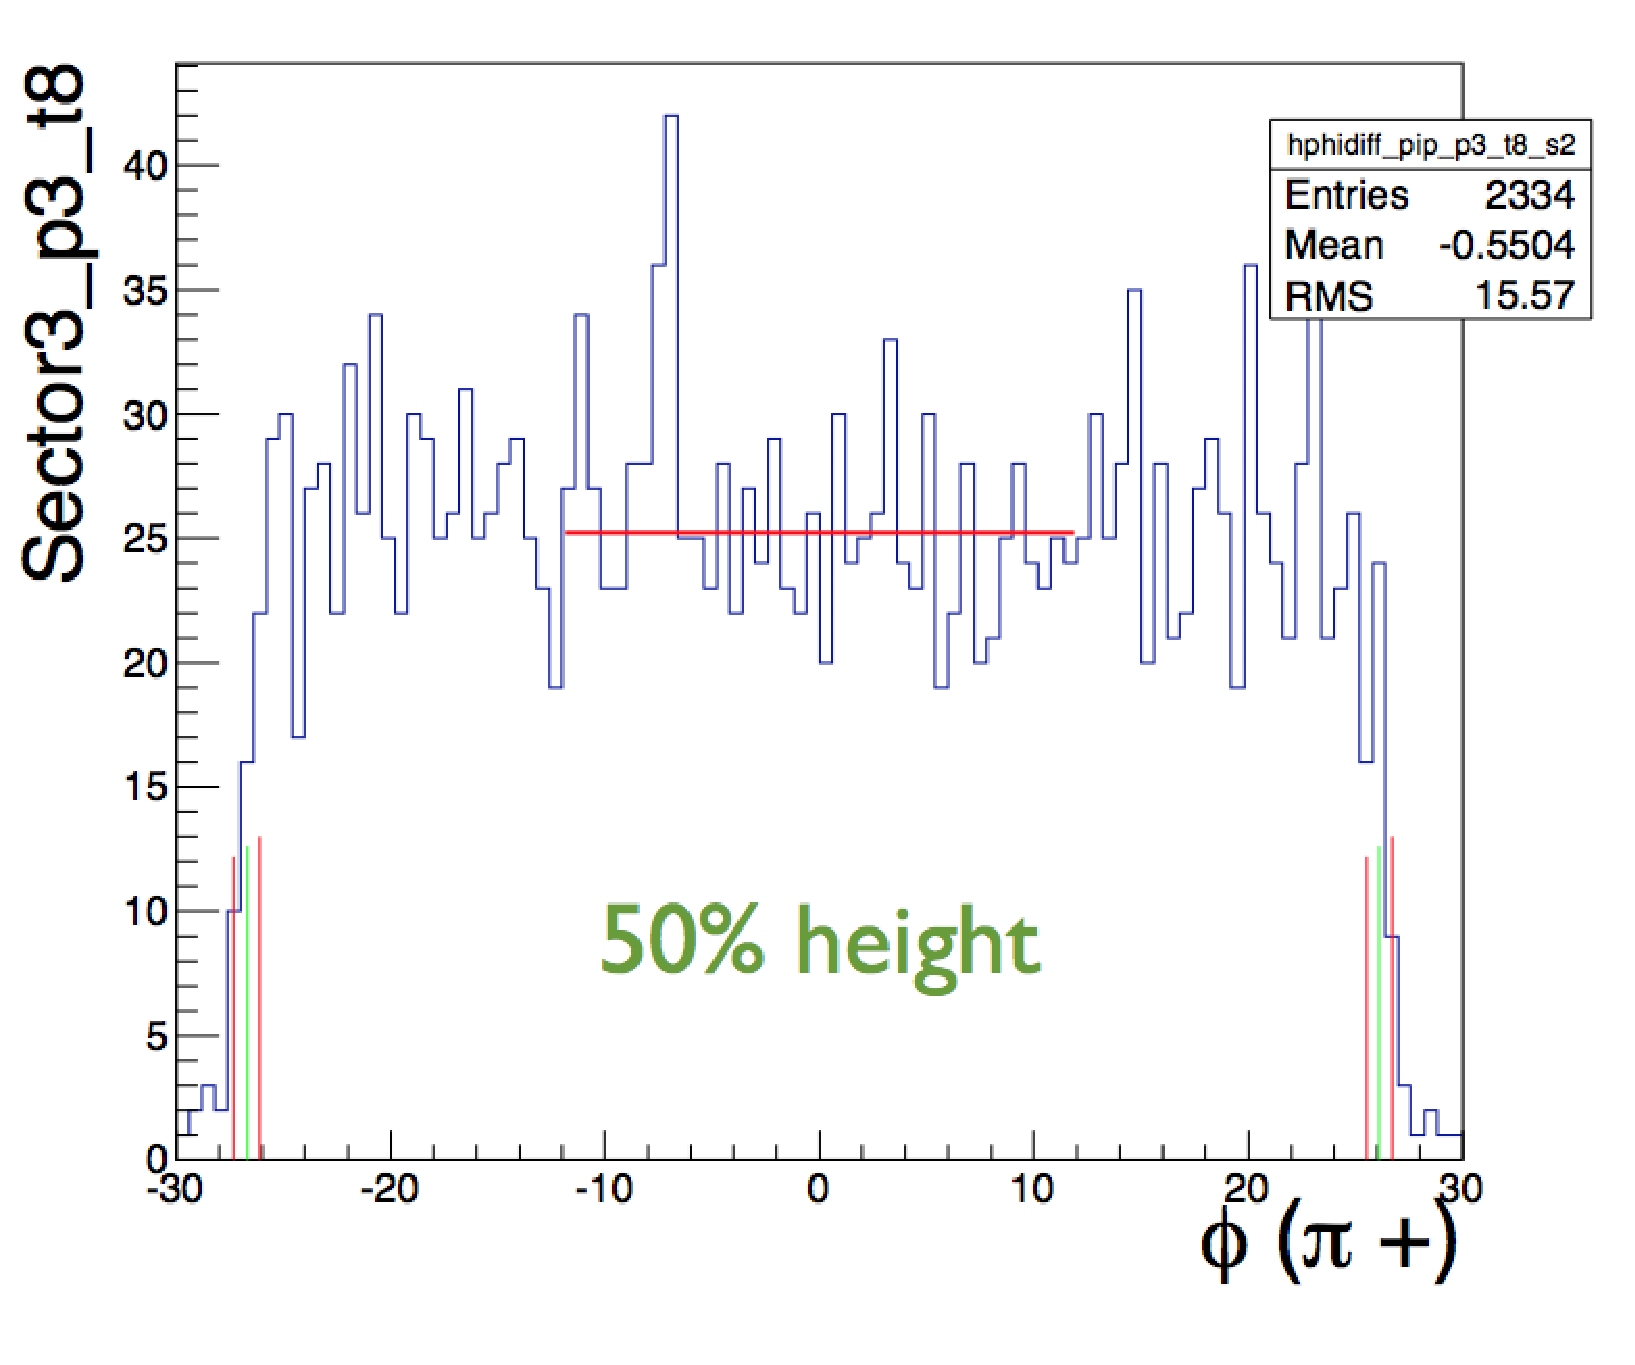
\includegraphics[width=0.48\linewidth]{figures/fiducial/gen1}
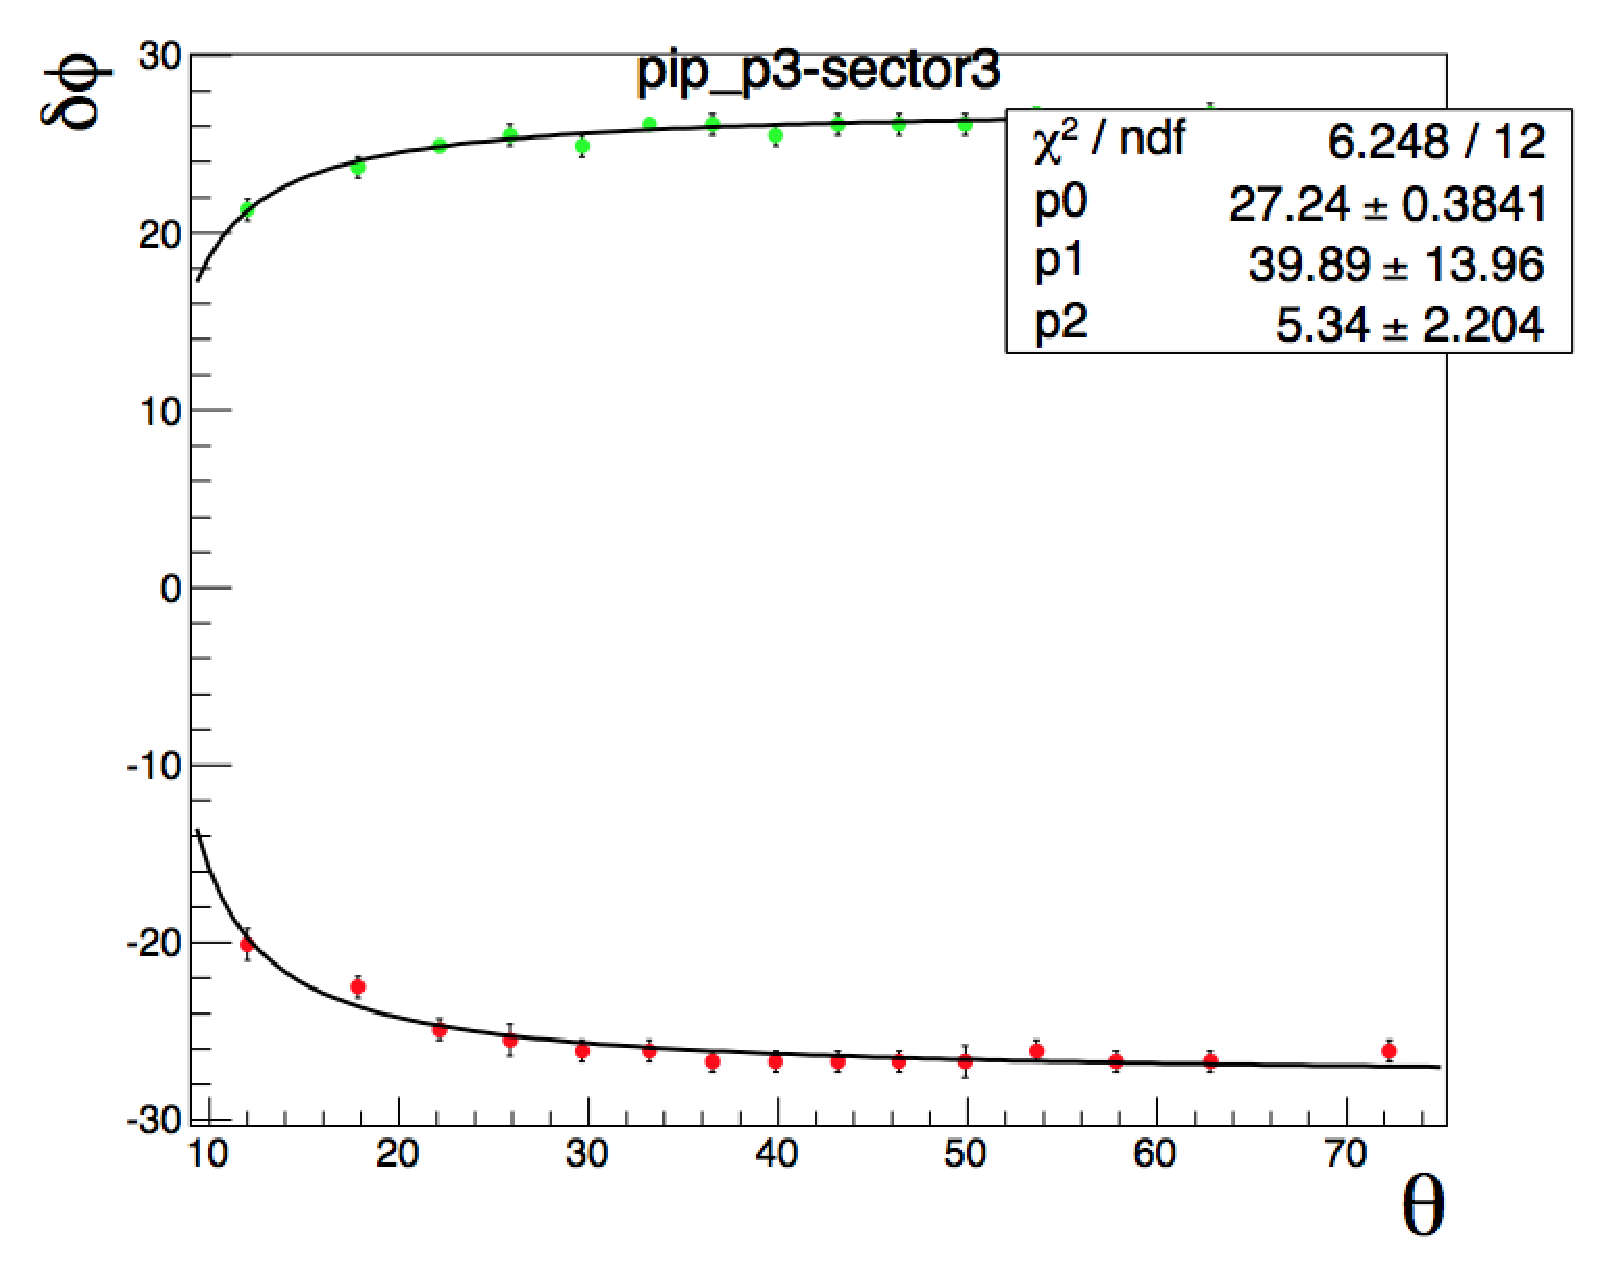
\includegraphics[width=0.48\linewidth]{figures/fiducial/gen2}
\caption{Left: shows the \π[+] $\phi$ distribution for sector-three in one $p$ and $\theta$ bin along with the upper and lower limits of the fiducial region represented by the green vertical line. Right: a second-generation plot, fit to a hyperbola.}
\label{gen12}
\end{figure}

\begin{figure}
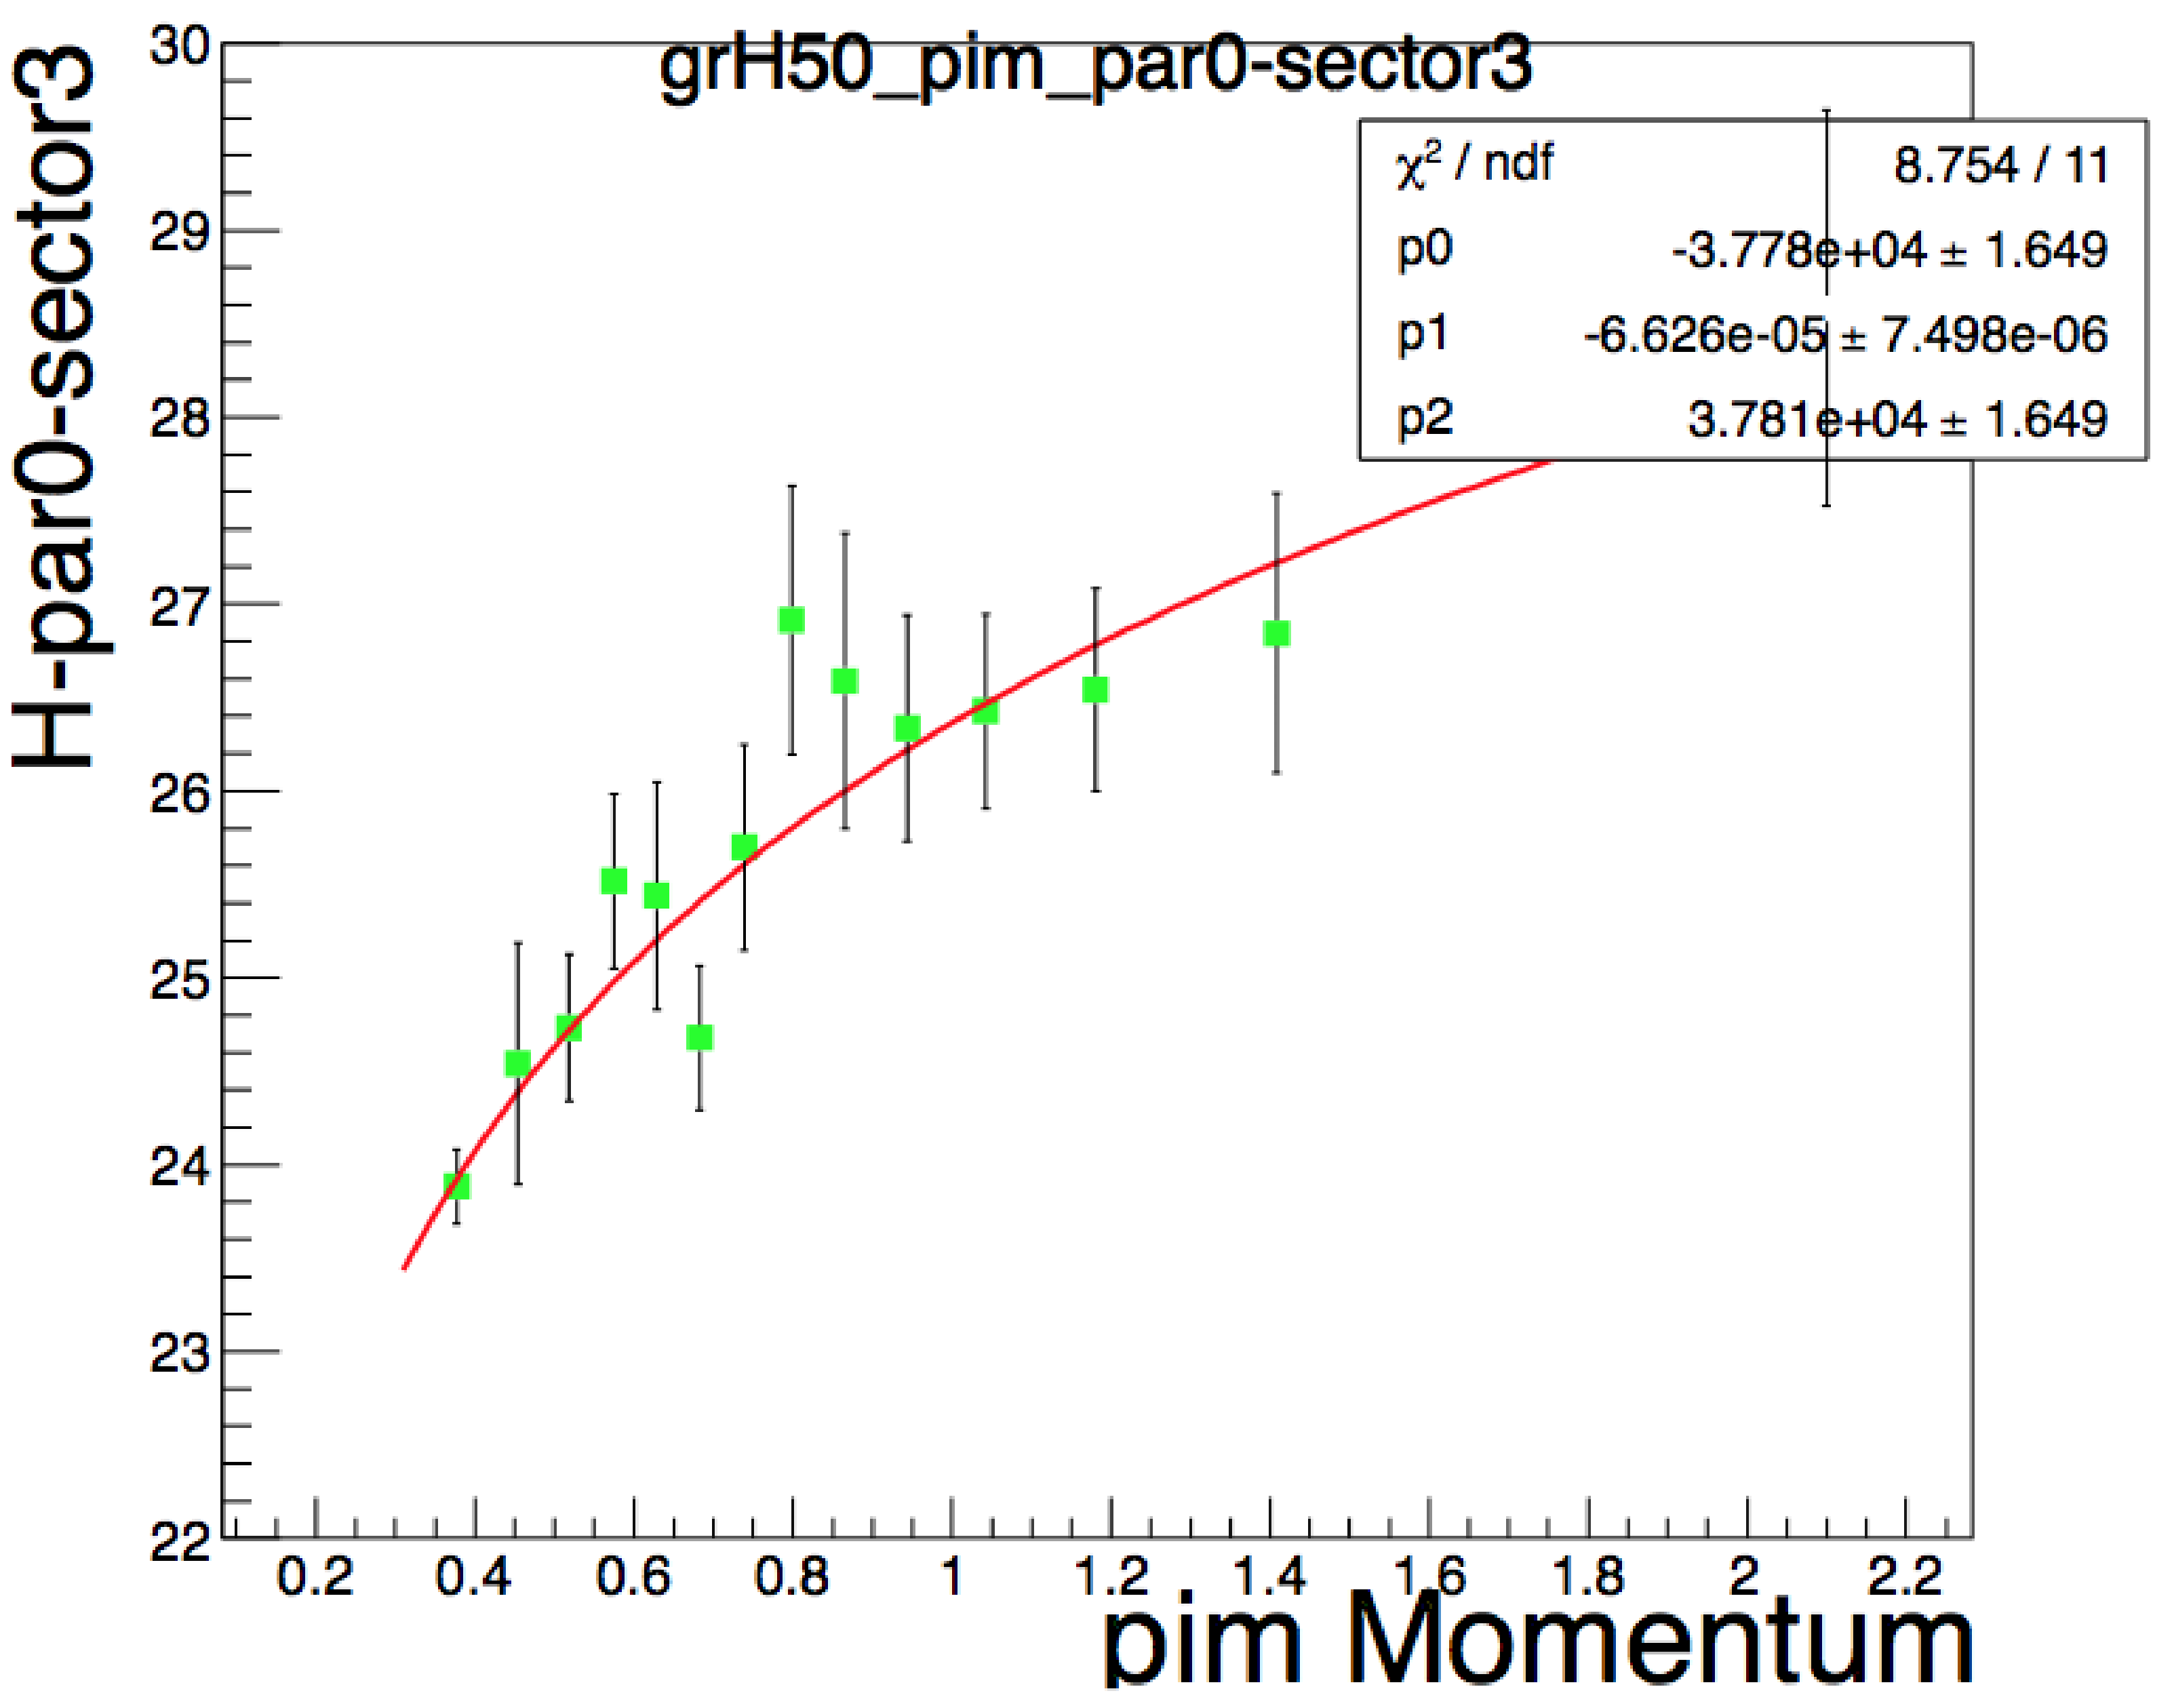
\includegraphics[width=0.48\linewidth]{figures/fiducial/3a}
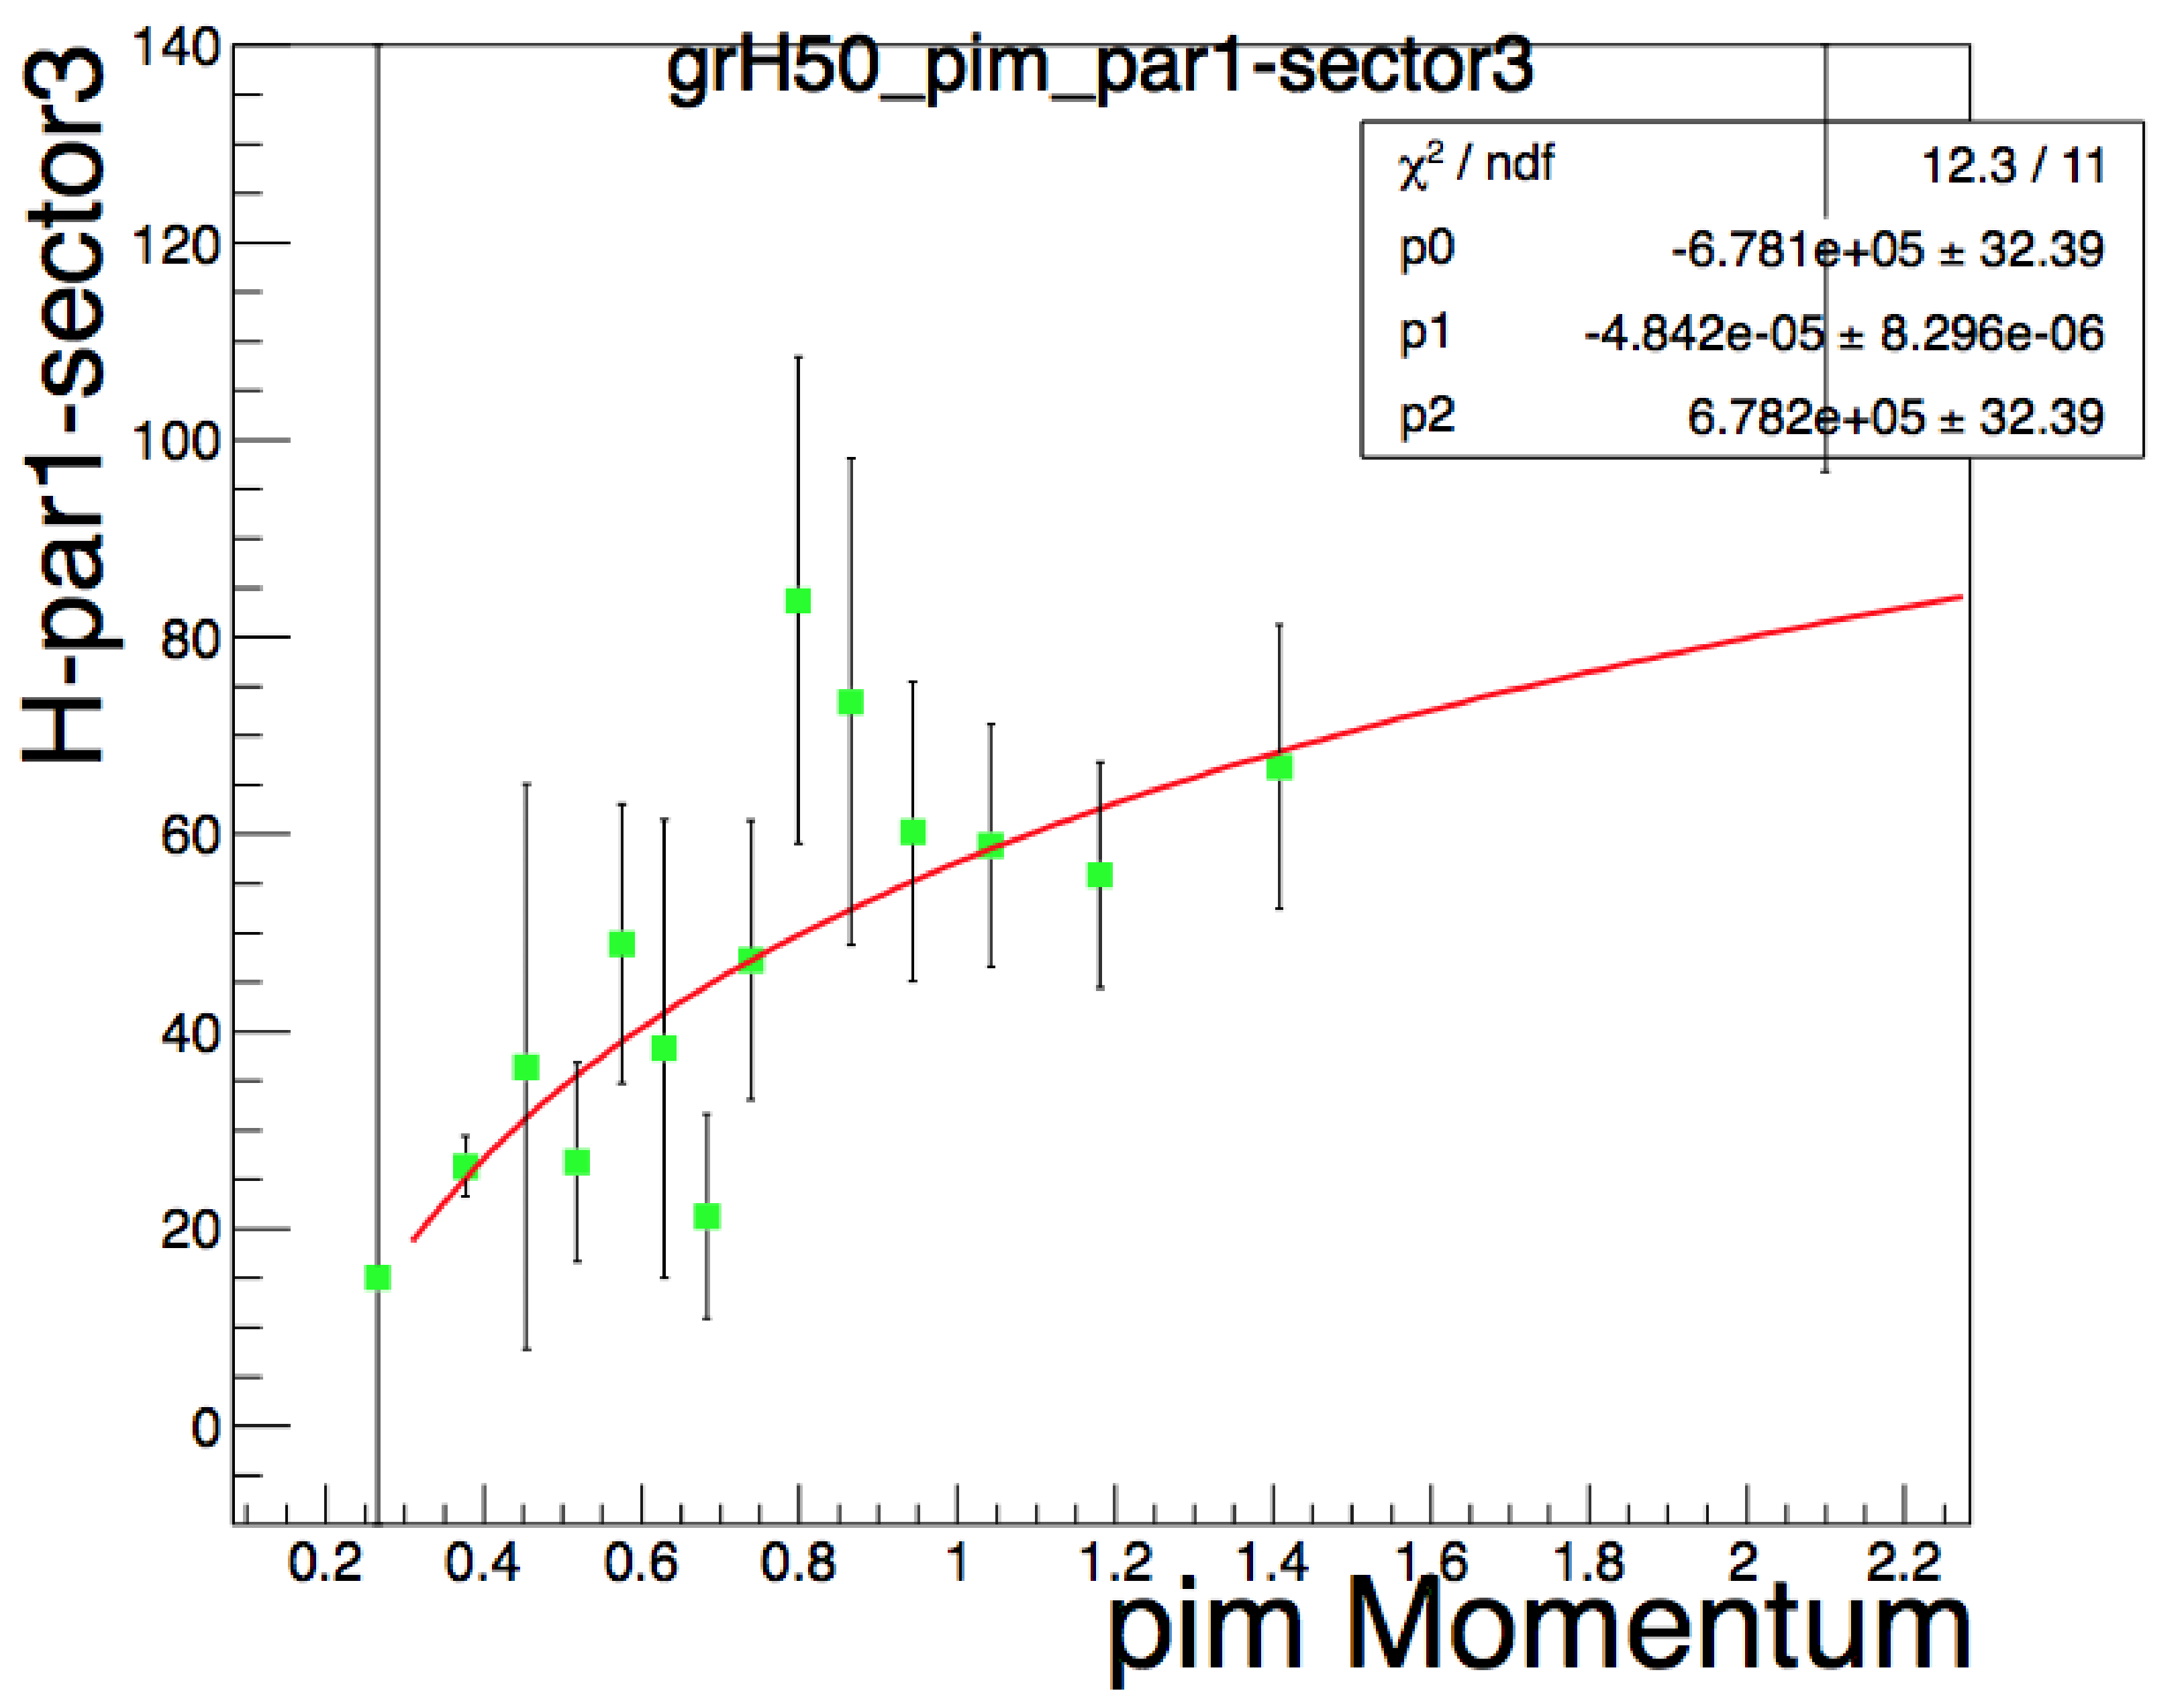
\includegraphics[width=0.48\linewidth]{figures/fiducial/3b}
\caption{Third-generation plots of the fitting parameters from second-generation fits for sector three. The data are fit to power functions.}
\label{gen3}
\end{figure}




\newcommand{\onefig}[3]{
\begin{figure}
    \centering
    \includegraphics[width=#1\textwidth]{#2}
    \caption{#3}
    \label{#2}
    \end{figure}
}


\onefig{0.6}{figures/fiducial/fid2}{The angular distribution of the proton from exclusive \mbox{p \π[+] \π[-]} events is shown.  In the top, $\phi$ vs $\theta$ is plotted, the bottom plots conveys similar information mapped to mimic the geometry of CLAS. Left: No fiducial cuts. Right: nominal fiducial cuts on the proton.}
\onefig{0.6}{figures/fiducial/fid3}{The angular distribution of the positive pion from exclusive \mbox{p \π[+] \π[-]} events is shown.  In the top, $\phi$ vs $\theta$ is plotted, the bottom plots conveys similar information mapped to reflect the geometry of CLAS. Left: no fiducial cuts. Right: nominal fiducial cuts on the positive pion.}
\onefig{0.6}{figures/fiducial/fid4}{The angular distribution of the negative pion from exclusive \mbox{p \π[+] \π[-]} events is shown.  In the top, $\phi$ vs $\theta$ is plotted, the bottom plots conveys similar information mapped to reflect the geometry of CLAS. Left: no fiducial cuts. Right: nominal fiducial cuts on the negative pion.}
\onefig{0.7}{figures/fiducial/fid5}{From left to right: $\phi$ vs momentum for the proton, negative pion and positive pion for \mbox{p \π[+] \π[-]} events. Top: no fiducial cuts. Bottom: nominal fiducial cuts.}
\newpage
To perform fiducial cuts for the G12 data use the header files:
\begin{verbatim}
https://jlabsvn.jlab.org/svnroot/clas/users/mkunkel/clas \
/g12_corrections/g12_NegParticle_fiducial_cuts.hpp
\end{verbatim}
and
\begin{verbatim}
https://jlabsvn.jlab.org/svnroot/clas/users/mkunkel/clas \
/g12_corrections/g12_PosParticle_fiducial_cuts.hpp
\end{verbatim}
The user needs the particle momentum, polar angle $\theta$, and azimuthal angle $\phi$. To use:
\begin{verbatim}
clas::g12:: \
g12_PosParticle_fiducial_cuts(particle_P, particle_Theta, particle_Phi,"nominal")
clas::g12::\
g12_NegParticle_fiducial_cuts(particle_P, particle_Theta, particle_Phi,"nominal")
\end{verbatim}
There are 3 types of options for the keyword depending on the desired cut, "nominal", "tight", and "loose". The header will return false if particle was not within fiducial region, true if particle was within fiducial region.
